\section{INTRODUCCIÓN}

\subsection{Marco y motivación del proyecto}

Las crisis alimenticias afectan a diversas partes del globo, en mayor o menor medida. Estas crisis pueden producirse por factores naturales o factores humanos como, por ejemplo, 
fallos en industrias, guerras, o, la que directamente se relaciona con este proyecto, agotamiento de los recursos naturales por la sobreexplotación.

Ante estas situaciones globales que pasan por revisar los valores de obtención de alimento y el cómo se gestionan los recursos, la pesca marítima está viendo como insostenible la 
compatibilidad de su labor con la generación de suficiente alimento vivo para suplir las necesidades exponenciales del ser humano.

El caso que más afecta a este trabajo es la acuicultura, un método alternativo que nació para obtener control sobre el desarrollo de especies muy difíciles de capturar en entornos 
libres. Esto se consigue a través de crianza controlada en entornos limitados, como piscifactorías o jaulas masivas en costas.

Este método de generación de alimento ha ido desarrollándose y mejorando a través de la introducción de nuevos métodos y tecnologías. Esta mejora ha permitido utilizar la acuicultura 
como principal método de crianza de ciertas especies, que; aun encontrándose en libertad, es más viable económicamente trabajar con ellas en estos entornos controlados. Esto permite liberar 
estrés de los ecosistemas marítimos.

Con estos ecosistemas tan afectados por las pescas de arrastre y, con la presión añadida por políticas limitantes en este ámbito, la pesca tradicional ha visto como la cantidad de alimento 
generado no crece a lo largo de los años. Esto se ve reflejado a través de los informes realizados por la \textit{\acrfull{fao}}, siendo el último en 2022, que marcaba aún más la tendencia del 
impulso hacia sistemas basados en acuicultura, observable en la \autoref{fig:EvolucionFAO}.

\begin{figure}[h]
    \centering
    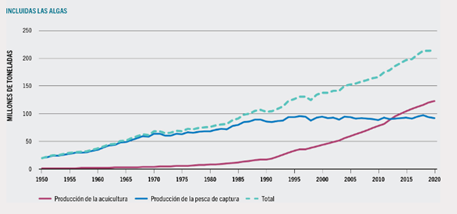
\includegraphics[width=0.75\textwidth]{images/2/EvolucionFAO.png}
    \caption{Evolución de la producción en la industria pesquera 1950-2020\cite{EstadoMundialPesca}}
    \label{fig:EvolucionFAO}
\end{figure}

La acuicultura está representando un cambio de paradigma para proteger nuestros ecosistemas y producir con menos perdidas y de manera más ética. Con esto en mente, se están 
promoviendo muchos planes de transformación digital en estas industrias, con la inversión en \acrshort{i+d} que eso conlleva.

Algunas de las investigaciones que se realizan en este campo tienen relación con el estudio de métodos de crianza que generen menos estrés en el pez. Mejoras en este campo podrían 
permitir un crecimiento más rápido del alimento vivo aumentando su bienestar y un mejor marco ético en la crianza del animal.

En concreto, para realizar un análisis y parametrizado del estrés del animal, se llevan a cabo diferentes experimentos con el objetivo final de valorar los resultados del cambio de metodologías. 
Siendo el \textit{NetTest}\cite{barriossanchezPruebaRedEvaluando2023} uno de estos experimentos.

El principal objetivo de este experimento es parametrizar la proactividad de un pez a través de los movimientos que realiza. Junto con este y otros datos del pez como podría ser su color o tamaño, 
intentar parametrizar y encontrar reglas de como se ha visto afectado por cambios de entorno. Si bien esta prueba no está estandarizada (la definición de movimiento puede variar entre diferentes 
trabajos académicos), en este trabajo se tratará el caso específico en el que los movimientos contados, son arpeos del espécimen.

En la actualidad esta prueba se realiza de forma manual, siendo necesario que el investigador utilice herramientas de análisis de videos para apuntar cuando se realizan estos movimientos, 
avanzando fotograma a fotograma. Un ejemplo de este tipo de herramientas son herramientas como BORIS\cite{friardBORISFreeVersatile2016}.

La existencia de este tipo de herramientas de código abierto es muy positiva para el mundo de la investigación, pero el hecho de tener un funcionamiento completamente manual conlleva un gasto 
de tiempo y recursos en obtener estos informes de movimientos para cada video.

Con esto en mente es interesante crear una alternativa que automatice el proceso de conteo de movimientos para los investigadores que utilizan el \textit{NetTest} como experimento principal.

\subsection{Objetivos técnicos y académicos}
Los objetivos de este trabajo consisten en:

\begin{itemize}
    \item Plantear una alternativa capaz de automatizar el \textit{NetTest}.
    \item Estudiar el uso de tecnologías basadas en procesado y análisis de imagen y técnicas de \textit{Deep Learning} para implementar esta alternativa.
    \item Desarrollar una aplicación completa a través de la alternativa planteada.
\end{itemize}

Los objetivos académicos de este proyecto son:

\begin{itemize}
    \item Desarrollar una mejor capacidad de análisis de requisitos técnicos a la hora de diseño de aplicaciones.
    \item Profundizar en el entendimiento de técnicas basadas en \textit{Deep Learning} como las redes neuronales.
    \item Mejorar las aptitudes relacionadas con el análisis de artículos académicos con el objetivo de realizar un estudio del arte suficientemente profundo, cohesionado y coherente con la problemática explicada.
\end{itemize}


\subsection{Estructura del resto de la memoria}
\todo[inline]{Falta hacer esta parte}